% file: pram-ar.tex

\documentclass[tikz]{standalone}

\usetikzlibrary{positioning, shapes, calc, backgrounds, fit}

\newcommand{\po}[2]{\draw [->, thick, violet] (#1) to node[above] {so} node[below, teal] {vis} (#2);}
\newcommand{\rw}[2]{\draw [->, thick, teal] (#1) to node[above, sloped, near end] {vis} (#2);}

\begin{document}
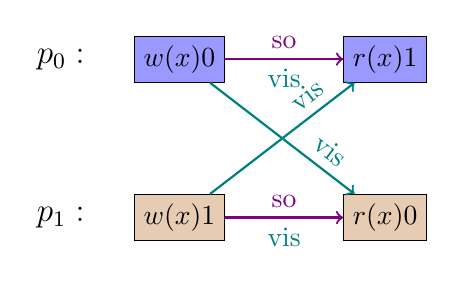
\begin{tikzpicture}[
    wop/.style = {rectangle, fill = blue!40, draw}, 
    rop/.style = {rectangle, fill = brown!40, draw}, 
    process/.style = {font = \large}]

  \node (p0) [process] {$p_0:$}; 
  \node (wx0) [wop, right = 0.5cm of p0] {$w(x)0$};
  \node (rx1) [wop, right = 1.5cm of wx0] {$r(x)1$};

  \node (p1) [process, below = 1.5cm of p0] {$p_1:$}; 
  \node (wx1) [rop, right = 0.5cm of p1] {$w(x)1$};
  \node (rx0) [rop, right = 1.5cm of wx1] {$r(x)0$};

  \po{wx0}{rx1}
  \po{wx1}{rx0}

  \rw{wx0}{rx0}
  \rw{wx1}{rx1}
\end{tikzpicture}
\end{document}
